\section{Theorie}
\label{sec:Theorie}
Der Photoeffekt beschreibt das Austreten von Elektronen aus einem Metall, welches mit Licht bestrahlt wird. Dabei treten Effekte auf, welche sich mit der Wellencharakteristik des Lichtes nicht erklären lassen.
So ist die maximale Kinetische Energie der Elektronen nicht etwa von der Intensität des bestrahlenden Lichtes, sondern nur von der Wellenlänge beziehungsweise der Frequenz des Lichtes abhängig. Des weiteren
tritt der Photoeffekt erst ab einer Grenzfrequenz auf. Dies lässt sich durch
Einführung der Photonen, aus welchen das Licht besteht, erklären. Der prinzipielle Aufbau des Photoeffektes ist in Abbildung \ref{fig:Prinzip} zu sehen.
\begin{figure}
  \centering
  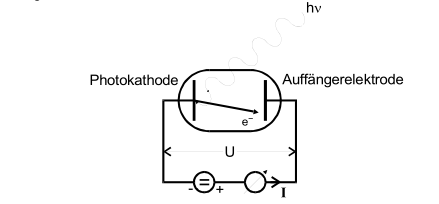
\includegraphics{images/Prinzip.png}
  \caption{Prinzipieller Aufbau des Photoeffektes \cite{sample}.}
  \label{fig:Prinzip}
\end{figure}
Die quantitative Beschreibung des Photoeffektes folgt aus der Energieerhaltung:
\begin{equation}
  h \nu = E_\text{kin} + A_k .
  \label{eqn:energie1}
\end{equation}
Dabei ist $h$ das Placksche Wirkungsquantum, $\nu$ die Frequenz des Lichtes, $E_\text{kin}$ die kinetische Energie des herausgelösten Elektrons und $A_k$ die Austrittsarbeit, die verrichtet werden muss um das Elektron aus dem
Festkörper zu lösen. Anhand dieser Energiebilanz werden die zuvor geschilderten Phänomene wie die Äbhangigkeit der kinetischen Energie von der Frequenz und die Grenzfrequenz für das Auftreten des Photoeffekts eindeutig beschrieben.
Da, wie im Folgenden Abschnitt \ref{sec:Durchführung} beschrieben, mit einer Gegenspannung, welche den durch Auftreffen der Elektronen auf die Anode entstehenden Strom ausgleicht, gearbeitet wird, muss die Energiebilanz angepasst werden.
Unter den Annahmen, dass die Energie der Bermspannung gleich der der schnellsten
Elektronen ist, und dass die Elektronen ihre Energie nur durch die Photonen erhalten haben, lässt sich folgende Gleichung aufstellen:
\begin{equation}
  h \nu = e_0 U_g + A_k .
  \label{eqn:energie2}
\end{equation}
Dabei ist $U_g$ die Bremsspannung und $e_0$ die Elementarladung der Elektronen.
Da die Elektronen im Festkörper jedoch eine nicht monoenergetische Energieverteilung besitzen, welche durch die Fermi-Dirac-Statistik beschrieben wird, verliert Gleichung \eqref{eqn:energie2} in der Praxis ihre Gültigkeit im Bezug auf
die Bremsspannung $U_g$. Die Elektronen besitzen im Festkörper Energien zwischen $0$ und der Fermi-Energie $\zeta$. Abhilfe verschafft die unter bestimmten Voraussetzungen geltende Beziehung
\begin{equation}
  I_\text{Ph} \sim U^2 .
  \label{eqn:ipropu}
\end{equation}
Besitzt die Anode jedoch eine sehr hohe Austrittsarbeit $A_A$ kann es sein, dass weitere Probleme bei der Untersuchung des Photoeffekts auftreten. Da die Kathode und Anode elektrisch leitend miteinader verbunden werden, stellen sich ihre
Fermi-Energien auf das selbe Niveau ein, wodurch teilweise eine Beschleunigungsspannung angelegt werden muss, um einen Photostrom zu messen. Dies ist anschaulich in Abbildung \ref{fig:AA} dargestellt.
\begin{figure}
  \centering
  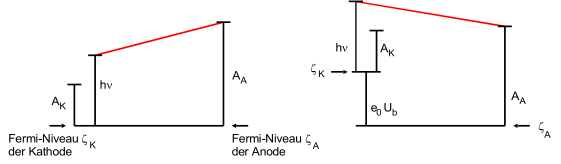
\includegraphics{images/AA.png}
  \caption{Beeinträchtigung des Photoeffekts durch hohe Austrittsarbeit der Anode \cite{sample}.}
  \label{fig:AA}
\end{figure}
